\documentclass[article]{aaltoseries}
\usepackage[utf8]{inputenc}

\begin{document}
 
%=========================================================

\title{Implementing a Virtual Network System among Containers}

\author{Songlin Jiang% Your first and last name: do _not_ add your student number
\\\textnormal{\texttt{songlin.jiang@aalto.fi}}} % Your Aalto e-mail address

\affiliation{\textbf{Tutor}: Tuomas Aura} % First and last name of your tutor

\maketitle

%==========================================================

\begin{abstract}
This paper investigates the method of implementing a virtual network system among containers. We implement a test environment for two types of VPN in IPv4: site-to-site, host-to-host, and site-to-site in IPv6. We compare Vagrant with VirtualBox as the provider and Docker Compose to realize the same functionality. The result shows that migrating the test from the Virtual Machines (VM) to the Docker containers can save nearly 90\% of CPU time and 94\% of memory for the VPN systems. At the same time, the host machine still has no security risk increase.

\vspace{3mm}
\noindent KEYWORDS: Container, Network, Cloud, VPN

\end{abstract}


%============================================================


\section{Introduction}

In recent years, container technologies, such as Docker, have received much attention from the industry and academia as applications are moving to the cloud. Containers are much more efficient and lightweight than virtual machines because containers share the Linux kernel with the host. In contrast, virtual machines employ hardware virtualization and have their own kernel instance, which consumes more resources \cite{10.1145/2988336.2988337}.

Virtual Private Networks (VPN) are typically used in complex networking environments with many different network components. It is still a common practice \cite{9151942} to build and test network systems using virtual machines, which allows the network engineer to experiment in a virtual environment before setting up the physical system. However, creating a virtual computing environment can also be slow and troublesome. The problems can worsen when testing VPN systems with a large number of nodes, as each network component and host needs a virtual machine instance. It can be memory-consuming to simultaneously run many virtual machine instances on one host machine to simulate the network environment, which significantly troubles testers working on personal computers due to short of memory. Moreover, Mac M1 / M2 chips are based on the ARM64 architecture, and virtual machine hypervisors currently have limited support for ARM64 hardware virtualization. However, ARM64 is well supported by container runtimes \cite{9852232}.

Containers are easy to launch on demand in the cloud, the cost is low because they can run within one virtual machine. Virtual networks are sometimes also needed for automated integration tests. Running with virtual machines can significantly increase the cost of Continuous Integration / Continuous Delivery (CI/CD) implementations in the cloud, as it's hard to use nested virtualization with limited resources. Furthermore, it is also hard to build, store and manage multi-platform virtual machine images in the cloud. At the same time, Docker supports building multi-platform images \cite{dockermultiplatform} and uploading them to Docker Hub.

Due to little research on implementing network systems using containers, this paper investigates the possibilities of implementing virtual network systems based on Docker containers to overcome the disadvantages of virtual machines, as mentioned above. This paper also analyzes the functional and security limitations when virtual networks are implemented this way.

This paper is organized as follows. Section 2 reviews the current technologies used for container networking. Section 3 defines our goal for implementing the VPN system using Docker containers, while Section 4 explains the details of our implementation. Section 5 presents our evaluation result by comparing the VPN system performance between the one implemented in the virtual machine and the one in the container. Finally, Section 6 provides the concluding remarks.

%============================================================


\section{Docker Networking System}
This section discusses the choice of the Docker container network driver for implementing the VPN system. It also discusses how to enable routing and firewalls inside a container.

\subsection{Network Drivers}
Docker employs a pluggable networking subsystem. Several drivers can provide the docker network functionality. The default drivers include the bridge, host, overlay, IPVLAN, MacVLAN, and none. We can choose one of them to implement the VPN system.

The none, host, and overlay drivers do not cater for our needs. Firstly, the none driver disables all networking. Secondly, the host driver is unnecessary, as it can cause security implications due to its nature of sharing the same network stack with the host machine. In addition, the overlay is not an appropriate option, as we are simulating the network system only on one host machine.

As a result, the possible candidates are bridge, IPVLAN, and MacVLAN. When examining the details, the bridge learns Media Access Control (MAC) addresses by checking the frame headers sent by the communicating hosts. At the same time, the MacVLAN is a trivial bridge that does not need to learn as it already knows every MAC address it can receive \cite{9620212}. IPVLAN is similar to MacVLAN, except MacVLAN assigns a different MAC address to each attached docker container. In contrast, IPVLAN assigns the same MAC address to all containers attached to it \cite{7502883}.

MacVLAN is the best choice for our needs. As we only use the driver to implement the internal network, there is no need to use advanced flood control and forwarding database manipulation that are specific to the bridge driver. Moreover, according to Docker documentation related to networking \cite{docker_documentation_2023}, MacVLAN networks are the best choice when migrating from a VM setup, as MacVLAN makes the container appear as a physical device with its own MAC address. Furthermore, Gundall et al. \cite{9442123} conduct benchmarks for different virtualization technologies for the networking overhead. The result shows that the MacVLAN driver performs best in throughput while requiring the least CPU resources compared to the other network drivers.

\subsection{Routing and Firewall}

By default, Docker containers do not allow manipulating container network devices and setting routing tables or firewalls inside the containers. These features can be enabled by assigning the net\_admin capability to the container.

According to the capabilities man page \cite{capabilities}, assigning the net\_admin capability to containers allows the following network-related operations:
\begin{enumerate}
\setlength{\itemsep}{0pt}
\setlength{\parsep}{0pt}
\setlength{\parskip}{0pt}
\item Interface configuration;
\item Administration of IP firewall, masquerading, and accounting;
\item Modifying routing tables;
\item Binding to any address for transparent proxying;
\item Setting the type-of-service (TOS);
\item Clearing driver statistics;
\item Setting the promiscuous mode;
\item Enabling multicasting;
\item Using setsockopt(2) to set the following socket options:
SO\_DEBUG, SO\_MARK, SO\_PRIORITY (for a priority outside the
range 0 to 6), SO\_RCVBUFFORCE, and SO\_SNDBUFFORCE.
\end{enumerate}

As we use the MacVLAN to build the internal network, all the network manipulations mentioned above only work for the network components that belong to the corresponding network namespace. There exist no security implications to the host network if we give net\_admin capability to the container that has its own network namespace.

\subsection{IPv6}
Configuring IPv6 networking in Docker \cite{docker_documentation_ipv6_2023} is also possible. Docker disables the IPv6 support by default. We can add the following content to the daemon configuration file (default location at: \texttt{/etc/docker/daemon.json}) or corresponding settings in Docker Desktop:

\texttt{\{
  "ipv6": true,
  "fixed-cidr-v6": "fd00::/80"
\}}

%============================================================


\section{Case Study: VPN}

This paper simulates a scenario where the IoT devices (clients) in two sites, A and B, would like to connect to the server in the cloud S. The topology is based on the Aalto University CS-E4300 Network Security 2022-2023 instance Project 2 \cite{aura_peltonen_bui_2022}, where site A, B, and cloud S both use the private IP address to improve the security and save the IPv4 address. Gateway A, B, and S connect site A, B, and S to the public Internet. The router in the topology is simplified, which routes across the Internet between the sites and the cloud. The address space between the gateway and the router simulates public, routable IPv4 addresses, although it is private. Site A, B, and cloud S use the router to access the Internet.

In order to make the clients in both site A and site B connect to the cloud server safely, this paper uses strongSwan, a VPN implementation based on Internet Protocol Security (IPsec).

This paper attempts to implement two types of VPN: site-to-site and host-to-host.

\subsection{Site to Site}
\begin{figure}[t!]
  \begin{center}
    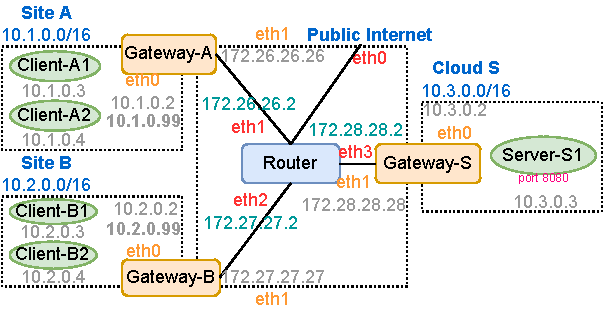
\includegraphics[width=1.1\textwidth]{figures/site-to-site.pdf}
    \caption{Site to Site}
    \label{fig:site2site}
  \end{center}
\end{figure}

A site-to-site VPN connects different network systems located at different sites together directly \cite{9022848}. In this case, the address spaces of sites A, B and the cloud network S should not overlap \cite{AKYILDIZ2023100695}.

Figure \ref{fig:site2site} shows the topology and corresponding address space under such circumstances.

\subsection{Host to Host}
\begin{figure}[t!]
  \begin{center}
    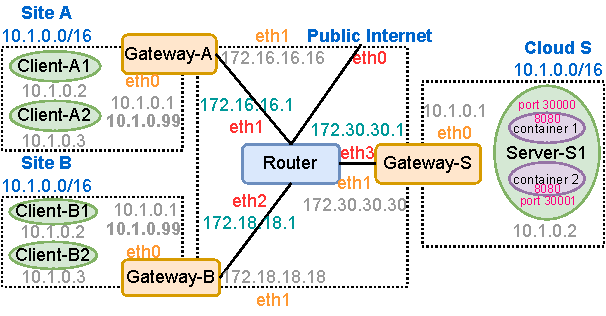
\includegraphics[width=1.1\textwidth]{figures/host-to-host.pdf}
    \caption{Host to Host}
    \label{fig:host2host}
  \end{center}
\end{figure}

A host-to-host VPN connects different gateways together. IP packets then get routed to different clients within the corresponding site according to the routing table of the gateway \cite{dulany2006performance}.

Figure \ref{fig:host2host} shows the topology and corresponding address spaces under such circumstances.

\subsection{Site to Site in IPv6}
\begin{figure}[t!]
  \begin{center}
    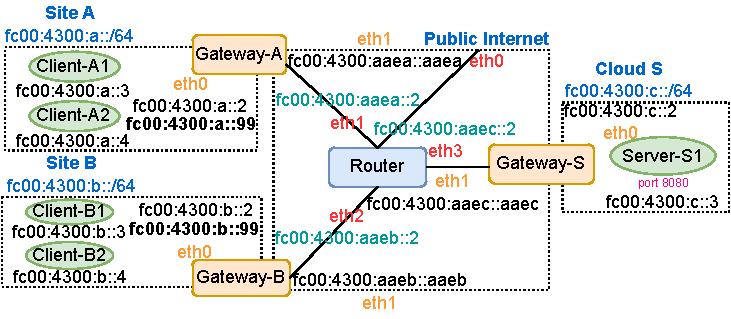
\includegraphics{figures/ipv6-site-to-site.pdf}
    \caption{Site to Site in IPv6}
    \label{fig:ipv6site2site}
  \end{center}
\end{figure}

Site to Site in IPv6 is similar to Site to Site VPN in IPv4 but replaces all the address space in IPv6.

Figure \ref{fig:ipv6site2site} shows the topology and corresponding address space under such circumstances.

%============================================================


\section{Implementation}

To manage the docker containers easily, we use Docker Compose to manage the orchestration. Based on the figures above, we make each network component a separate container, assign the net\_admin capability to each container, and implement the network with the MacVLAN driver. We only connect the router to the docker default bridge network to simulate the public Internet. Finally, we set up the routing and firewall and configure the strongSwan IPsec correctly with certificates.

For routing, we use Network Address Translation (NAT) masquerade for the gateway interface in order to prevent leaking local IP addresses outside their subnets. We bind the IP address 10.1.0.99 to the interface eth0 of gateway A and 10.2.0.99 to B.

We use strict firewall rules on the clients, assuming there should be no need for the clients (IoT devices) to visit the Internet. We use iptables to set up gateway A and B firewall rules for input and output. We accept Internet Key Exchange (IKE) and Encapsulating Security Payload (ESP) traffic (port 500 and 4500 in UDP) from and to the cloud. Finally, we drop everything else, including the connection from and to the Internet.

There are also some differences between the two kinds of VPN setup as well as between the IPv4 and IPv6 one:

\subsection{Site to Site}

Concerning routing, for gateway A and B, we redirect the traffic from the local address (10.1.0.99 and 10.2.0.99) of port 8080 to cloud server S1 on port 8080 with Destination NAT.

For the firewall on gateway A and B, we also have to accept the post-routing traffic to the cloud server 10.3.0.3.

There is no overlapping network address space within the site-to-site VPN, thus we can specify the IP address and subnet directly through Docker Compose. Additionally, we avoid using the IP address ending in ".1", as Docker does not allow us to assign that address to any container. These addresses are reserved for gateways or routers on a particular network (although we are simulating the Gateway and Router).

\subsection{Host to Host}

About routing, for gateway A and B, we redirect the traffic from the original local server address 10.1.0.99 of port 8080 to cloud gateway S of port 8080 with Destination NAT. For gateway S, we redirect the traffic from the client gateway A and B of port 8080 to corresponding ports (30000 and 30001) on the server s1 address.

There are overlapping network address spaces for host-to-host VPN. Suppose we specify the IP address and subnet directly through Docker Compose. In that case, there will be errors notifying us that 'Pool overlaps with another one on this address space'. Although technically this should not be a problem as we are creating a separate internal network without direct routing, Docker still forbids us.

We have addressed the issue of overlapping address space through a method that can be likened to IP address spoofing. When we do not specify the IP address of the network in Docker Compose, it will assign a random address from the docker address pool to the network interface. Now we can modify the IP address and subnet of the interface to our desired one, and no error will be thrown now.

In addition, for server S1, we use the Docker-in-Docker image to run docker containers inside the server S1 container. Running that image requires the container to be privileged according to the documentation \cite{Docker}. As a result, in practice, we must ensure the software running in server S1 is benign and poses no risk to the host machine. It can be acceptable in a testbed network but not in production. Otherwise, we recommend having a separate VM for the servers.

\subsection{Site to Site in IPv6}

Site to Site in IPv6 is similar to Site to Site in IPv4. Just replacing all the IPv4 addresses with IPv6 would complete the job. The only difference is that, in addition to the existing configurations, we also have to allow ICMPv6 traffic at the gateways for firewall rules. In IPv6, Neighbor Discovery is a necessary component, replacing Address Resolution Protocol (ARP) in IPv4. This way, IPv6 Neighbor Discovery can work, and different containers can communicate within their subnet. We also need ICMPv6 for Destination Unreachable messages.

%============================================================

\section{Evaluation}
\subsection{Performance}
We use Docker Engine 23.0.1 to run the containers and VirtualBox 7.0.6 to run the Virtual Machines. The table \ref{tab:result} reflects the average situation for all the 3 implementations.

\begin{table}[t!]
  \begin{center}
    \begin{tabular}{|l|lr|}
    \hline
    Solution               & Boot Time$^1$ & Memory$^2$ \\
    \hline
    Docker Compose         &   75 s    &  278 MB \\
    Vagrant + VirtualBox   &  689 s    &  4.5 GB \\
    \hline
    \end{tabular}
    \caption{Performance Test Result in Average}
    \label{tab:result}
  \end{center}
\end{table}

The table \ref{tab:result} shows that our container solution significantly reduces the fresh boot time\footnote{Also include the running environment building time for the host platform} for the whole VPN system by nearly 90\%. It also dramatically reduces the memory consumption\footnote{Maximum value during the whole running process} by nearly 94\% as well.

\subsection{Security and Benefits}
We can check the current virtual network devices with the command \texttt{ls /sys/devices/virtual/net -l}. It shows different results when executing from the host machine and inside the container, indicating that the network stacks inside containers are entirely isolated from the host machine.

The shell script commands for making all the related routing and firewall configurations in Docker containers and VMs are identical, hence migrating configurations from the VMs to the docker containers is easy. We can simultaneously start the site-to-site and host-to-host VPN setup in Docker without interfering with each other.

We can also use Docker buildx \cite{dockermultiplatform} to create the testing environment images for multiple platforms with only one machine, then upload to Docker Hub for easy reuse, while VMs do not allow us to do so.

Most importantly, the docker setup can run in M1/M2 based macOS easily with docker desktop, while the VM ones fail to start.

\subsection{Limitations}

There are also some limitations of the Docker networking model, which cause several observable differences compared to VMs. However, in general, these limitations all have workarounds to bypass and will not stop us from adopting container solutions.

\begin{enumerate}
\setlength{\itemsep}{0pt}
\setlength{\parsep}{0pt}
\setlength{\parskip}{0pt}
\item We are not allowed to assign the IP address ending in ".1" to a Docker container, while we will only get a warning if we do that in a VM.
\item We cannot have overlapped IP addresses assigned by Docker, the only way to do that is to configure manually inside containers.
\end{enumerate}

In addition, if we want to test the scalability of the network software and run docker containers inside a docker container, that container needs to be privileged, which may cause some security risks, but this is not necessary for implementing virtual networks.

%============================================================


\section{Conclusion}

This paper investigates the method to construct the testing environment of the VPN system through Docker containers. Containers are much more lightweight than virtual machines. As a mature virtualization technology, containers can realize every functionality we require, similar to virtual machines in our case, while increasing no security risk to the host machine.

We hope this paper can inspire researchers and engineers to migrate their testing environment related to network systems from VMs into containers.

Source code for this paper: \textit{https://github.com/HollowMan6/Implement-VPN-System-with-Containers/tree/main/src}

%============================================================


% \section{Simple things first}

% In this section, we give some simple examples of Latex mark-up.
% Sec.~\ref{sec:emphasis} emphasizes important points and
% Sec.~\ref{sec:math} gives examples of math formulas.
% Finally, \ref{sec:list} demonstrates lists.


% %------------------------------------------------------------


% \subsection{Emphasizing text}
% \label{sec:emphasis}

% \textit{Italics} is a good way to emphasize printed text. However,
% \textbf{boldface} looks better when converted to HTML.

% Paragraphs are separated by an empty line in the Latex source code.
% Latex puts extra space between sentences, which you must suppress
% after a period that does not end a sentence, e.g.\ after this acronym.

% Cross-references to figures (Fig.~\ref{fig:mypicture1}), tables
% (Table~\ref{tab:mytable1}), other sections (Sec.~\ref{sec:math})
% are easy to create. 


% %------------------------------------------------------------


% \subsection{Mathematics}
% \label{sec:math}

% In the mathematics mode, you can have subscripts such as $K_{master}$
% and superscripts like $2^x$. Longer formulas may be put on a separate
% line:
% \[ \emptyset \in \emptyset \; \Rightarrow \; E \neq mc^2. \]

% You may also want to number the formulas like Eq.~(\ref{eqn:myequation1})
% below.
% \begin{equation}\label{eqn:myequation1}
% C = E_{K_{public}}(P) = P^e. \hspace{10mm}   P = D_{K_{private}}(C) = C^d.
% \end{equation}



% %------------------------------------------------------------


% \subsection{Make a list}
% \label{sec:list}

% Lists can have either bullets or numbers on them. 

% \begin{itemize}
% \item one item
% \item another item, which is an exceptionally long one for an item
%   and consequently continues on the next line.
% \end{itemize}

% Lists can have several levels. Item~\ref{kukkuu} below contains
% another list.
% \begin{enumerate}
% \item the fist item \label{kukkuu}
%   \begin{enumerate}
%   \item the first subitem 
%   \item the second subitem
%   \end{enumerate}
% \item the second item
% \end{enumerate}


% %============================================================


% \section{More complex stuff}

% This section provides examples of more complex things.


% %------------------------------------------------------------


% \subsection{Data served on a table}


% Table~\ref{tab:mytable1} presents some data in tabular form. 

% \begin{table}[t!]
%   \begin{center}
%     \begin{tabular}{|l|lr|}
%     \hline
%     Protocol & Year &  RFC \\
%     \hline
%     TCP      & 1981 &  793 \\
%     ISAKMP   & 1998 & 2408 \\
%     Photuris & 1999 & 2522 \\
%     \hline
%     \end{tabular}
%     \caption{A table with some protocols}
%     \label{tab:mytable1}
%   \end{center}
% \end{table}


% %------------------------------------------------------------


% \subsection{Adding references}
% \label{sec:references}

% Do not forget to give pointers to the literature. If you are listing
% stuff related to your topic, you can give several references once
% \cite{Com00,HTS03,Nik99}. However, usually you should give only one, for example the standard describing the stuff \cite{RFC2408} and if you want to directly use someone else's words, use both quotation marks and refer to the source, for example that ``the developer does not need to know all about the framework to develop a working implementation'' \cite{Suo98}. Remember also to mark references to your pictures if they are not created by your own mind!

% If you plan to write with Latex regularly, create your own BibTeX
% database and use BibTeX to typeset the bibliographies automatically.
% In the long run, it will save you a lot of time and effort compared to
% compiling reference lists by hand.


% %------------------------------------------------------------


% \subsection{Embedded pictures}
% \label{sec:pictures}

% Fig.~\ref{fig:mypicture1} is an embedded picture. The supported formats for pictures
% depend on the actual LaTeX command used. For instance, regular \LaTeX supports
% pictures in EPS (Embedded PostScript) format, while pdf\LaTeX supports PDF (Portable
% Document Format), PNG (Portable Network Graphics) and JPEG (Joint Photographic Experts
% Group). It is recommended to use either EPS or PDF for diagrams as well as for any picture
% which includes vector images.

% \begin{figure}[t!]
%   \begin{center}
%     % Note how the file extension has been removed from the filename below
%     % so that the LaTeX command can automatically pick any supported file format
%     \includegraphics[width=.5\textwidth]{figures/sample}
%     \caption{An embedded picture}
%     \label{fig:mypicture1}
%   \end{center}
% \end{figure}


% %============================================================


% \section{Yet another section title}

% To be added.


%============================================================


\bibliographystyle{plain}
\bibliography{cs-seminar}

\end{document}
